

\chapter{Migratory birds stopped visiting Aral}
\label{cp:aral-birds}

\begin{figure}[htbp]
  \centering
  \begin{minipage}[b]{0.45\textwidth}
    \centering
    \fbox{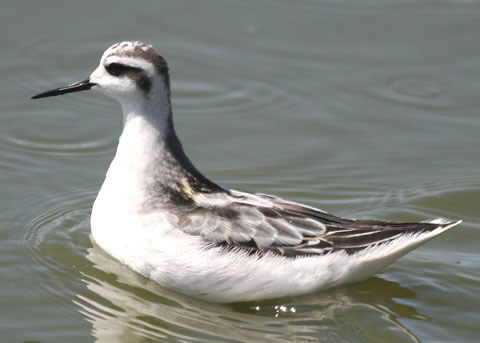
\includegraphics[width=0.8\textwidth]{Figures/Appendices/Aral Phalarope.png}}
    \caption{Aral Phalarope}
    \label{fig:aral-phalarope}
  \end{minipage}
  \hfill
  \begin{minipage}[b]{0.45\textwidth}
    \centering
    \fbox{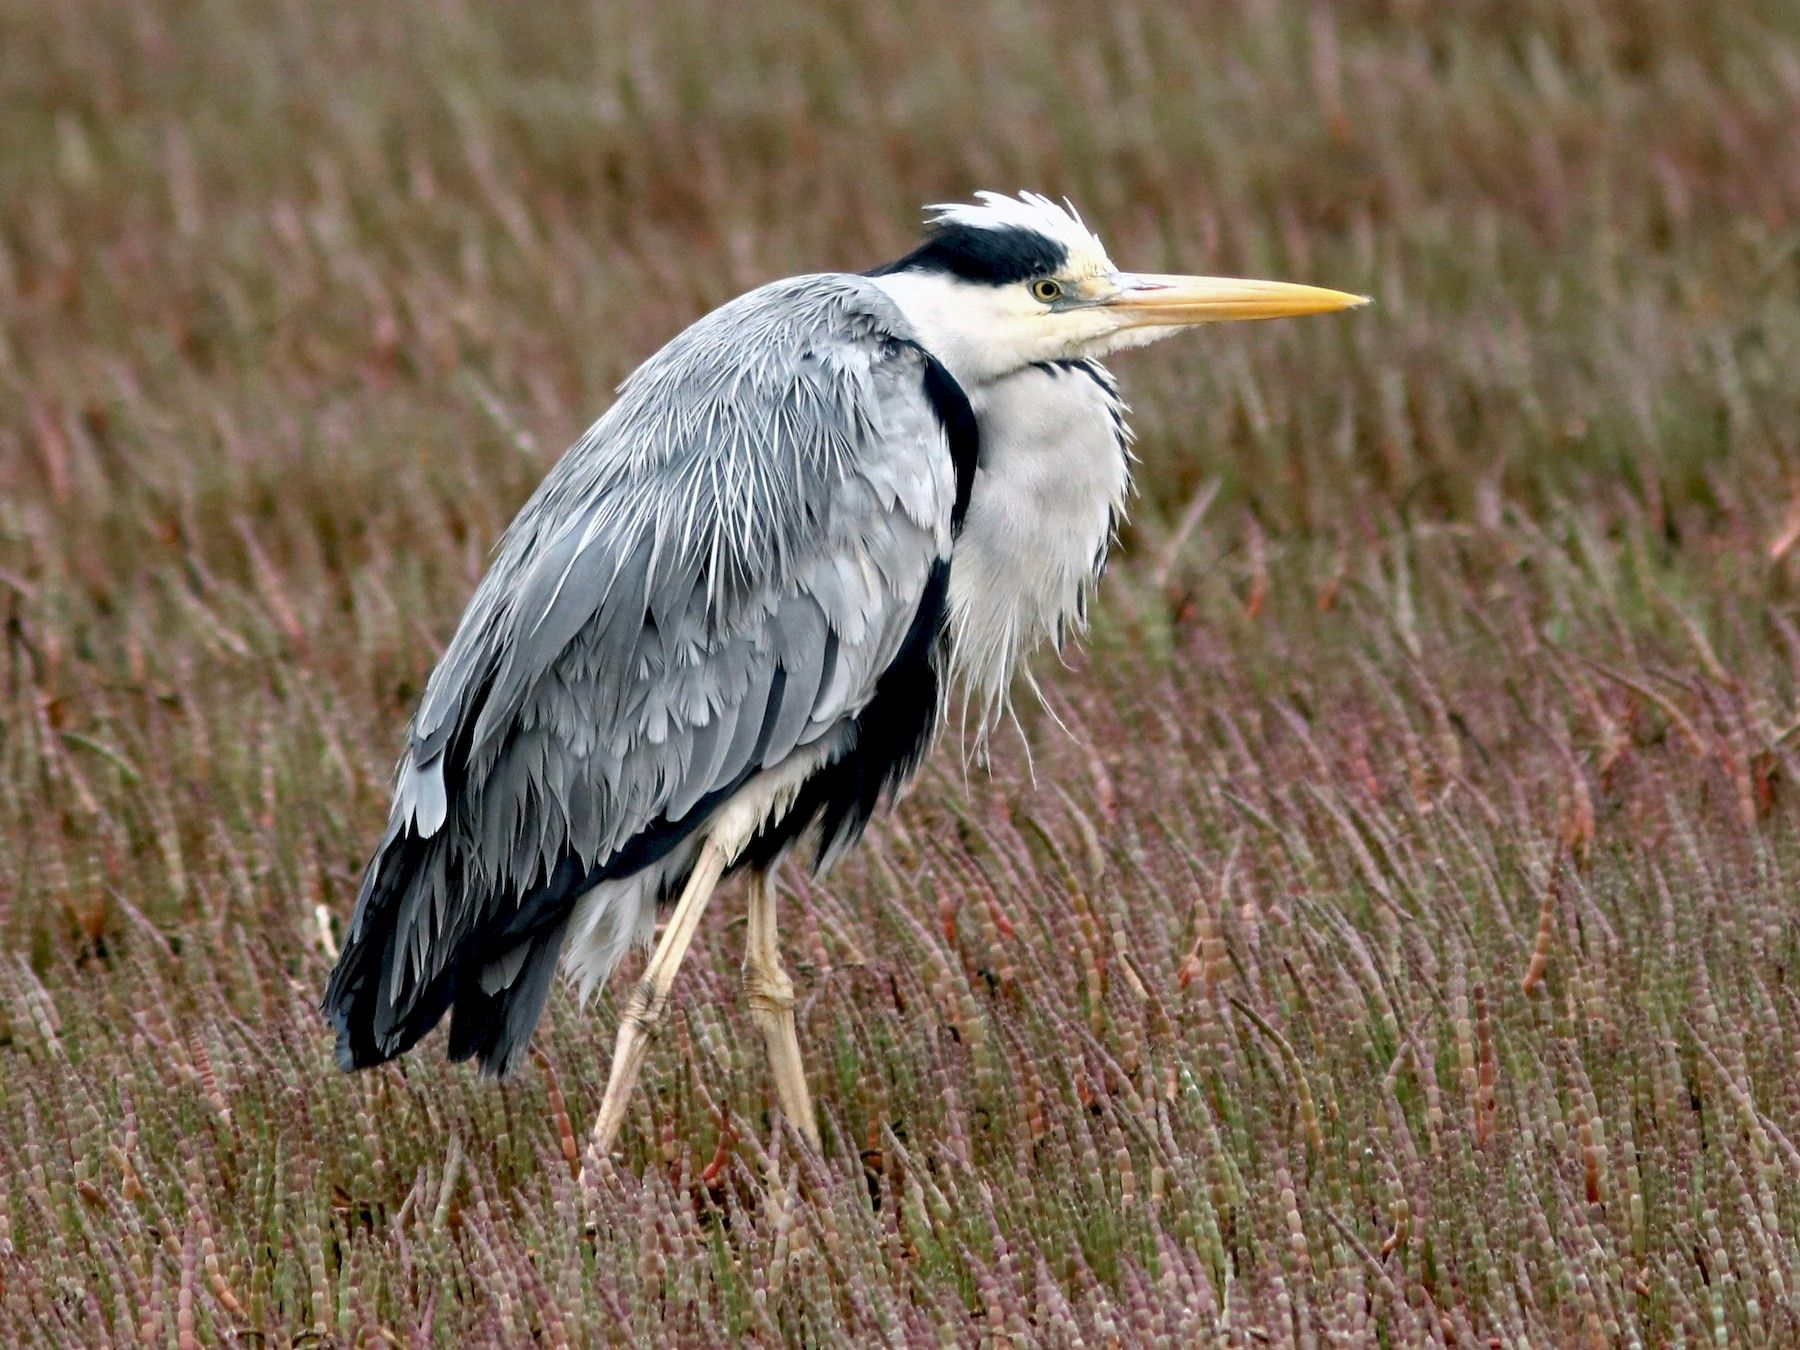
\includegraphics[width=0.8\textwidth]{Figures/Appendices/grey-heron.png}}
    \caption{Grey Heron}
    \label{fig:heron}
  \end{minipage}
\end{figure}

\begin{figure}[htbp]
  \centering
  \begin{minipage}[b]{0.45\textwidth}
    \centering
    \fbox{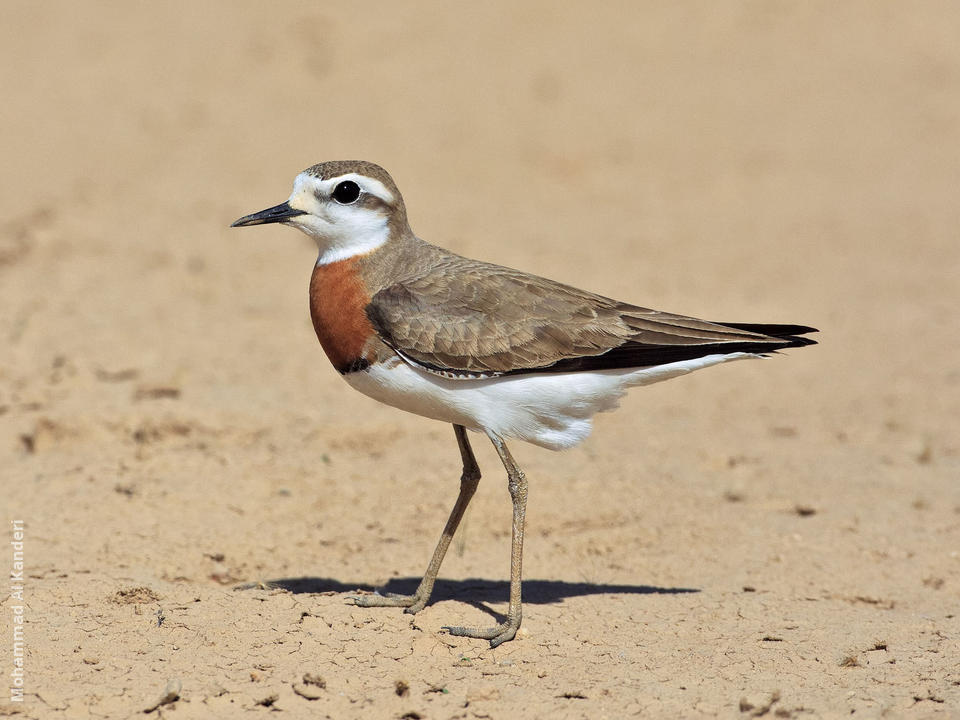
\includegraphics[trim=0mm 0mm 0mm 20mm, clip, width=0.8\textwidth]{Figures/Appendices/caspian plover.jpg}}
    \caption{Caspian Plover}
    \label{fig:}
  \end{minipage}
  \hfill
  \begin{minipage}[b]{0.45\textwidth}
    \centering
    \fbox{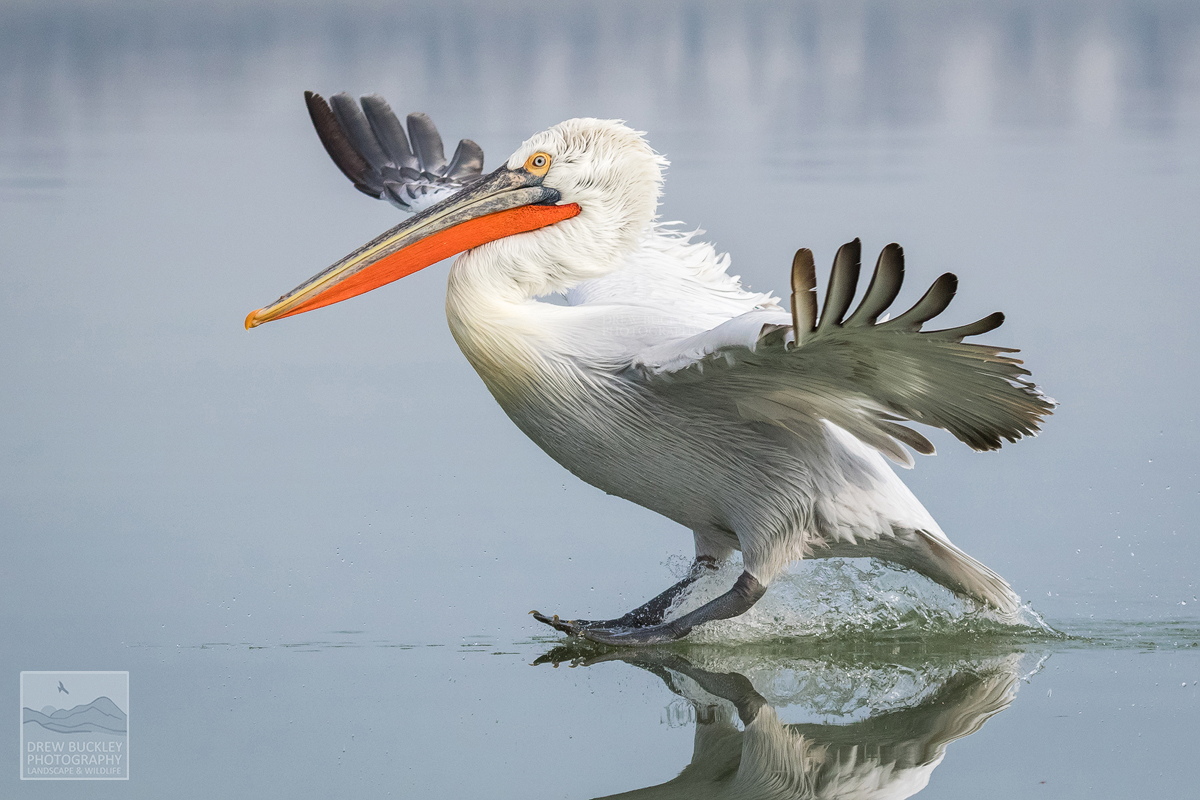
\includegraphics[width=0.8\textwidth]{Figures/Appendices/dalmation pelican.jpg}}
    \caption{Dalmation Pelican}
    \label{fig:}
  \end{minipage}
\end{figure}

\begin{figure}[htbp]
  \centering
  \begin{minipage}[b]{0.45\textwidth}
    \centering
    

    \fbox{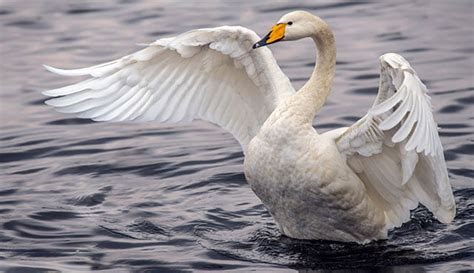
\includegraphics[width=0.8\textwidth]{Figures/Appendices/whooper-swan.png}}
    \caption{Whooper Swan}
    \label{fig:whooper-swan}
  \end{minipage}
  \hfill
  \begin{minipage}[b]{0.45\textwidth}
    \centering
    \fbox{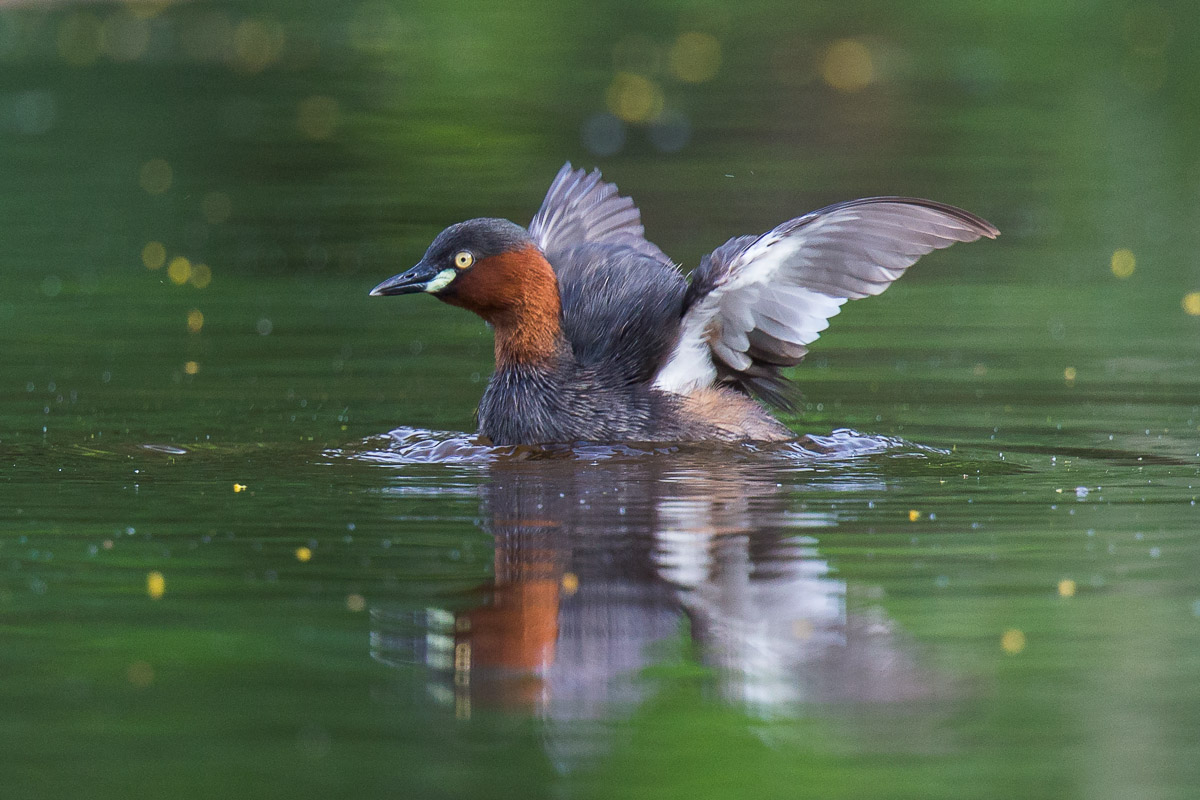
\includegraphics[width=0.8\textwidth]{Figures/Appendices/little grebe.jpg}}
    \caption{Little Grebe}
    \label{fig:}
  \end{minipage}
\end{figure}


\begin{table}[h]
\centering
\caption{Migratory breeding bird species and rare winter visitors}
\begin{tabular}{ll}
\hline
\textbf{Group} & \textbf{Species} \\
\hline
Wetland-dependent birds & Mute swan (\textit{Cygnus olor}) \\
& Mallard (\textit{Anas platyrhynchos}) \\
& Gadwall (\textit{Anas strepera}) \\
& Caspian gull (\textit{Larus cachinnans}) \\
\hline
Coastal and island plain inhabitants & Black-bellied sandgrouse (\textit{Pterocles orientalis}) \\
& Pallas’s sandgrouse (\textit{Syrrhaptes paradoxus}) \\
& Lesser short-toed lark (\textit{Calandrella rufescens}) \\
& Calandra lark (\textit{Melanocorypha calandra}) \\
& Shore lark (\textit{Eremophila alpestris}) \\
\hline
Coastal and island outcrop inhabitants & Ruddy shelduck (\textit{Tadorna ferruginea}) \\
& Shelduck (\textit{Tadorna tadorna}) \\
& Jackdaw (\textit{Corvus monedula}) \\
& Rock sparrow (\textit{Petronia petronia}) \\
\hline
\end{tabular}
\end{table}

\begin{table}[h]
\centering
\caption{Resident breeding bird species}
\begin{tabular}{ll}
\hline
\textbf{Group} & \textbf{Species} \\
\hline
Plain inhabitants & Gray partridge (\textit{Perdix perdix}) \\
& Crested lark (\textit{Galerida cristata}) \\
& Pander’s ground jay (\textit{Podoces panderi}) \\
\hline
Riparian forest inhabitants & Common pheasant (\textit{Phasianus colchicus turcestanicus}) \\
& White-winged woodpecker (\textit{Dendrocopos leucopterus}) \\
& Magpie (\textit{Pica pica}) \\
& Turkestan tit (\textit{Parus bokharensis}) \\
\hline
Coastal outcrop inhabitants & Golden eagle (\textit{Aquila chrysaetos}) \\
& Barbary falcon (\textit{Falco pelegrinoides babylonica}) \\
& Eagle owl (\textit{Bubo bubo}) \\
& Little owl (\textit{Athene noctua}) \\
& Raven (\textit{Corvus corax}) \\
\hline
Inhabitants of settlements & Rock dove (\textit{Columba livia}) \\
& Collared dove (\textit{Streptopelia decaocto}) \\
& Laughing dove (\textit{Streptopelia senegalensis}) \\
& House sparrow (\textit{Passer domesticus}) \\
& Tree sparrow (\textit{Passer montanus}) \\
\hline
\end{tabular}
\end{table}

